\documentclass[conference]{IEEEtran}
\IEEEoverridecommandlockouts

\usepackage{cite}
\usepackage{amsmath, amssymb, amsfonts}
\usepackage{graphicx}
\usepackage{textcomp}
\usepackage{booktabs}
\usepackage{url}
\usepackage[hidelinks]{hyperref}

\graphicspath{{figures/}}

\def\BibTeX{{\rm B\kern-.05em{\sc i\kern-.025em b}\kern-.08em T\kern-.1667em\lower.7ex\hbox{E}\kern-.125emX}}

\begin{document}

\title{The Disparate Impact of Knowledge Distillation\\
on Membership Privacy}

\author{
  \IEEEauthorblockN{Tejas Gulur}
  \IEEEauthorblockA{
    Department of Electrical and Computer Engineering\\
    University of Washington\\
    Seattle, WA, USA\\
    \texttt{tgulur@uw.edu}
  }
}

\maketitle

\begin{abstract}
Knowledge distillation is widely treated as a privacy-friendly compression technique. The student is trained on teacher logits rather than on raw labeled records, and population-level membership inference accuracy drops sharply after distillation. On the Texas-100X healthcare dataset, the loss-based attack of Yeom et al.\ achieves an AUC of $0.642$ on a moderately overfit teacher and collapses to $0.529$ on a distilled student of the same architecture family. That number is the kind that gets cited as evidence that distillation reduces leakage, but it hides a very uneven distribution of residual risk. On the highest-loss quartile of training samples the student still leaks an AUC of $0.89$ and a true-positive rate of $76\%$ at a $1\%$ false-positive rate, against $0.96$ and $87\%$ on the teacher. An independent Feldman and Zhang memorization estimator, computed from held-out reference models, recovers the same pattern. Student true-positive rates on memorized samples sit between $7\%$ and $30\%$ across mitigations, a worst-case leakage rate one to two orders of magnitude above the population mean. The asymmetry parallels the argument Bagdasaryan et al.\ made against differential privacy. A privacy intervention whose benefit accrues predominantly to the population that was already safe is not delivering the guarantee its evaluation implies.
\end{abstract}

\begin{IEEEkeywords}
membership inference, knowledge distillation, privacy auditing, disparate impact, healthcare machine learning, Texas-100X
\end{IEEEkeywords}

\IEEEPARstart{K}{nowledge} distillation is most familiar as a model-compression technique, but it is also studied as a privacy mechanism. The student is trained only on the teacher's soft outputs rather than on raw labeled records, and the standard intuition is that this indirection should reduce membership inference leakage. The supporting evidence in this line of work is almost always a single number. Population-level attack AUC drops sharply after distillation, and the conclusion is drawn that the resulting model leaks less.

That argument is incomplete in a way that matters for healthcare deployments. Membership inference is, in practice, a per-record threat. An attacker who learns that an average patient in a hospital's training set is no longer identifiable does not benefit. An attacker who learns that the small number of patients with rare procedures or unusual feature combinations remain identifiable does. If the privacy gain from distillation is concentrated on the easy, common samples that were never very vulnerable in the first place, while the long-tail samples retain almost all of their leakage, then the population AUC is not measuring the privacy property that an operator would actually care about. It is averaging over the patients for whom the question never had any teeth.

This paper asks whether that is the case on a realistic healthcare dataset, and what common knowledge-distillation-side mitigations do about it. The pipeline below implements a tabular teacher, a distilled student, and three mitigation variants on Texas-100X, and runs three established membership inference attacks against each. The population result reproduces the canonical distillation-reduces-AUC finding. The same scores, stratified along three independent subgroup signals, tell a much more uneven story. One of the signals is per-sample teacher loss, one is class frequency, and one is a Feldman and Zhang memorization score computed from held-out reference models. The memorization signal is included specifically to address the partial circularity of stratifying by loss when the attack itself uses loss as its score. Under all three the same pattern reproduces. The population view substantially understates residual leakage on the worst-case subsets, and mitigations that look essentially identical at the population level diverge by an order of magnitude on the memorized long tail.

\section*{Background and Related Work}

Membership inference itself has a well-developed literature. The shadow-model framework of Shokri et al.~\cite{shokri2017} trains auxiliary models on data drawn from the same distribution as the target and learns to discriminate in-set from out-of-set membership from the target's output distribution. Yeom et al.~\cite{yeom2018} observed that the per-sample loss is itself often a near-optimal membership signal when the model exhibits a generalization gap, and the loss-based attack has become the standard baseline. Carlini et al.~\cite{carlini2022} reframed the problem as a per-sample likelihood ratio test (LiRA) and made the more significant methodological argument that the appropriate evaluation metric is not the ROC AUC but the true-positive rate at low false-positive rates. The policy-relevant question is whether an attacker can confidently flag any record at all, not whether the attacker can sort records better than chance on average.

Distillation has been pitched as a defense against this class of attack~\cite{shejwalkar2021, tang2022}. The argument is that the student never trains on the raw membership-labeled records, only on teacher logits, so the student should leak less. The evidence is typically aggregate AUC reduction reported on the population.

Bagdasaryan et al.~\cite{bagdasaryan2019} demonstrated that differentially private training disproportionately damages accuracy on underrepresented subgroups. A privacy technique's cost, in other words, can be unevenly distributed. The analogous question for the \emph{benefit} of a privacy technique has been raised for federated learning but not, on the available literature, for knowledge distillation. The framing here is the contrapositive of the Bagdasaryan critique. A privacy intervention whose benefit accrues to those who needed protection least is not delivering meaningful privacy.

Feldman and Zhang~\cite{feldman2020} define per-sample memorization as the causal effect of inclusion in training on the model's correctness at that sample. Their definition takes the form
\begin{equation*}
  \mathrm{mem}(x) = \Pr[h(x) = y \mid x \in S] - \Pr[h(x) = y \mid x \notin S]
\end{equation*}
and is estimated empirically by training many models on random subsets and averaging in-set against out-of-set correctness per sample. The estimator depends only on the reference models, not on the target model or on any specific attack score. That independence is what makes it the right tool for the circularity problem discussed in the evaluation.

\section*{Approach}

Texas-100X is a tabular dataset of $924{,}954$ patient records drawn from $441$ Texas hospitals~\cite{texas100x}. The prediction task is to classify the principal surgical procedure code from a small set of demographic and admission features. The \texttt{THCIC\_ID} hospital identifier is excluded from model inputs to prevent trivial leakage of the originating institution. The label set is restricted to the top $100$ most frequent procedure codes. Splits are deterministic at $50{,}000$ training records, $10{,}000$ validation records, and $50{,}000$ test records, and all attacks target the training set as the membership set.

The label distribution is heavily long-tailed even after the restriction to the top $100$ codes. The two most frequent codes together account for $12.4\%$ of records, the $22$ codes in the $1\%$ to $5\%$ range cover $51.3\%$, and the $76$ codes individually under $1\%$ make up the remaining $36.3\%$. The rare-class subgroup that appears throughout the subgroup analysis is therefore an aggregate over $76$ procedure codes rather than a thin slice of the population, which is what makes the subgroup statistically large enough to estimate AUC and a low-FPR TPR on.

The teacher is a tabular multi-layer perceptron with categorical embeddings, hidden dimensions $[512, 512, 256]$, dropout $0.05$, trained for $75$ epochs of AdamW with a step learning-rate schedule. The distilled student shares the input pipeline but uses a smaller backbone of $[256, 256, 128]$ hidden units. It is trained for $50$ epochs with the standard Hinton distillation loss at temperature $T=4$, and the weighting $\alpha$ on the hard cross-entropy term is chosen from a sweep over $\{0.3, 0.5, 0.7\}$. Three mitigation variants reuse the student backbone with a single intervention each. The first is a rank $32$ linear bottleneck on the input projection. The second removes batch normalization layers entirely. The third is a data-side mitigation. The top $10\%$ of training samples by teacher confidence are dropped before the student sees them, on the intuition that the most-confident teacher samples are also the ones the teacher overfit on, and so excluding them from the distillation set should reduce the privacy signal the student inherits. Confidence here is the maximum softmax probability of the teacher over the predicted class, taken at the model's native temperature without rescaling. The $10\%$ cutoff is used as a default and was not tuned, so a sensitivity sweep on the cutoff is one of the natural follow-ups.

The attack suite has three pieces plus a fourth for completeness. The loss-based attack of Yeom et al.\ assigns each sample a score equal to the negative per-sample cross-entropy loss, so higher scores correspond to predicted membership. The shadow-model attack of Shokri et al.\ trains four shadow models on disjoint subsets of held-out data and learns a meta-classifier on the target model's output distribution. An approximate Likelihood Ratio Attack fits in-set and out-of-set Gaussian distributions on the target model's own confidence statistics, a cheaper variant of the full LiRA construction. The full LiRA is run too, with $K = 64$ reference models each trained on a random $50\%$ subsample for $5$ epochs. Those reference models double as the substrate for the Feldman and Zhang memorization estimator below. The behavior of the full LiRA at this value of $K$ is taken up under limitations.

For each combination of model, attack, and mitigation, the attack scores are binned by three subgroup signals, and AUC and true-positive rate at $1\%$ false-positive rate are computed per bin. Class-frequency bins are defined by label frequency in the training set. A label appearing in fewer than $1\%$ of training records is \emph{rare}, $1\%$ to $5\%$ is \emph{medium}, and more than $5\%$ is \emph{common}. The loss-quantile stratification uses quartiles $q_1$ through $q_4$ of per-sample teacher loss. The memorization stratification uses fixed thresholds on the Feldman and Zhang score, with the high-memorization bin defined as $\widehat{\mathrm{mem}}(x) > 0.3$. Quantile binning does not work for memorization because the empirical distribution clusters at zero, and quartile boundaries collapse into the noise floor.

The subsample-based estimator of Feldman and Zhang is used to compute $\widehat{\mathrm{mem}}(x)$. Each of the $64$ LiRA reference models contributes one in-set observation if the sample was in its training subsample and one out-of-set observation otherwise, and $\widehat{\mathrm{mem}}(x)$ is computed as the difference of mean correctness across the two groups. With $50\%$ subsampling and $64$ reference models, each target sample has approximately $32$ in-set and $32$ out-of-set observations. The estimator is biased relative to the strict leave-one-out definition (the paper analyzes this directly), but the sample-level ranking, which is what the stratification depends on, is preserved. Critically, the memorization signal is derived from the reference models' argmax correctness, not from the target model's loss, and it is therefore independent of both the target model and the attack score used in evaluation.

\section*{Evaluation}

Table~\ref{tab:population} presents the population-level membership inference results. The teacher overfits substantially, producing a $16$-point generalization gap that the loss-based attack readily exploits at an AUC of $0.642$. The distilled student closes most of the gap on average, and the same attack on the student drops to an AUC of $0.529$, a result consistent with the existing distillation-as-defense literature. Population true-positive rates at the $1\%$ false-positive threshold are near $1\%$ across all student variants, essentially indistinguishable from random performance at that operating point. The full LiRA row at $K = 64$ reference models is included in the same table for completeness, but the $0.503$ AUC sits well below the loss-based and approximate-LiRA results and should not be interpreted as substantive evidence about the teacher's leakage. The cause is a known sample-complexity issue with the full attack at small $K$, taken up under limitations.

\begin{table*}[t]
\caption{Population-level membership inference results. $50{,}000$-record training set, seed $509$. Test accuracy is reported as train then test.}
\label{tab:population}
\centering
\footnotesize
\setlength{\tabcolsep}{8pt}
\begin{tabular}{llrrr}
\toprule
Model & Attack & AUC & TPR @ $1\%$ FPR & Train / Test Acc.\ \\
\midrule
Teacher & loss-based & $0.642$ & $1.2\%$ & $63.6\% / 47.4\%$ \\
Teacher & approx-LiRA & $0.652$ & $1.8\%$ & $63.6\% / 47.4\%$ \\
Teacher & full LiRA ($K{=}64$) & $0.503$ & $1.3\%$ & $63.6\% / 47.4\%$ \\
\midrule
Student (none) & loss-based & $0.529$ & $1.1\%$ & $39.4\% / 37.8\%$ \\
Student (bottleneck) & loss-based & $0.523$ & $1.1\%$ & $39.3\% / 37.7\%$ \\
Student (no-BN) & loss-based & $0.512$ & $1.1\%$ & $34.9\% / 35.2\%$ \\
Student (conf-filter) & loss-based & $0.524$ & $1.1\%$ & $38.4\% / 38.0\%$ \\
\bottomrule
\end{tabular}
\end{table*}

Read in isolation, this table supports the standard claim that distillation reduces population-level membership leakage, and that the three mitigations stacked on top of distillation are essentially equivalent to plain distillation in their effect. Both halves of that reading are the subject of the discussion that follows.

Binning the same attack scores by per-sample teacher loss changes the picture substantially. On the highest-loss quartile the loss-based attack against the teacher achieves an AUC of $0.963$ and a true-positive rate of $87.2\%$ at $1\%$ FPR. The student variants on the same quartile sit between $0.88$ and $0.90$ AUC and between $75\%$ and $77\%$ TPR. The population gap between teacher and student was about $0.11$ AUC. On the worst quartile, that gap is $0.07$. Class-frequency stratification points the same direction (Table~\ref{tab:freq}). Rare-class samples sit at an attack AUC of $0.69$ on the student loss-based attack, against $0.20$ for samples from common classes. The population AUC of $0.53$ turns out to be an artifact of the well-classified, high-frequency majority that were never meaningfully vulnerable, and it says very little about the long-tail patients and rare conditions the teacher actually memorized.

\begin{table}[t]
\caption{Loss-based attack metrics stratified by procedure-code frequency. Rare classes account for under $1\%$ of training records each and together cover the long tail of the procedure-code distribution. AUC monotonically decreases with class frequency for both target models, and the absolute leakage on the rare bin is more than three times the leakage on the common bin for the student.}
\label{tab:freq}
\centering
\footnotesize
\begin{tabular}{lrrrrr}
\toprule
& & \multicolumn{2}{c}{Teacher} & \multicolumn{2}{c}{Student} \\
\cmidrule(lr){3-4} \cmidrule(lr){5-6}
Bin & $n$ & AUC & TPR & AUC & TPR \\
\midrule
rare ($<1\%$)        & $36{,}489$ & $0.723$ & $0.6\%$ & $0.686$ & $0.5\%$ \\
medium ($1\%$ to $5\%$) & $51{,}140$ & $0.636$ & $1.3\%$ & $0.494$ & $1.6\%$ \\
common ($>5\%$)      & $12{,}371$ & $0.427$ & $4.2\%$ & $0.204$ & $2.1\%$ \\
\bottomrule
\end{tabular}
\\[2pt]
{\footnotesize TPR is reported at the $1\%$ FPR operating point.}
\end{table}

The loss-quartile result has a circularity problem. The loss-based attack's score is, up to sign, the per-sample loss itself, so binning samples by loss and observing that the high-loss bins exhibit high attack AUC partially confirms the binning criterion rather than constituting an independent finding. The prior progress report on this project identified the concern explicitly and named the Feldman and Zhang memorization scores as the natural external signal.

The empirical memorization distribution, estimated from $64$ reference models, clusters heavily at zero. Feldman and Zhang predict exactly this shape for long-tailed datasets. Of the $100{,}000$ target samples evaluated, $196$ fall into the high-memorization bin defined by $\widehat{\mathrm{mem}}(x) > 0.3$. On this bin the student's loss-based attack AUC drops below $0.5$. The reason is that the student does not actually memorize most of the samples the reference models memorize. Its loss on a memorized member is no longer monotonically related to membership, and the AUC inverts. The metric that survives this inversion is true-positive rate at low false-positive rate, which picks up the small fraction of memorized samples the student \emph{did} memorize even when the bulk are mis-ranked.

\begin{table}[t]
\caption{Subgroup metrics on the Feldman and Zhang high-memorization bin ($\widehat{\mathrm{mem}}(x) > 0.3$, loss-based attack). The teacher and student bins each contain $49$ samples per mitigation. Population numbers from Table~\ref{tab:population} are included for contrast.}
\label{tab:fz}
\centering
\footnotesize
\begin{tabular}{lrr}
\toprule
Model / mitigation & AUC & TPR @ 1\% FPR \\
\midrule
Teacher, \texttt{mem\_high} & $0.635$ & $0.0\%$ (small $N$) \\
Teacher, population & $0.642$ & $1.2\%$ \\
\midrule
Student / none, \texttt{mem\_high} & $0.397$ & $\mathbf{18.5\%}$ \\
Student / bottleneck, \texttt{mem\_high} & $0.340$ & $\mathbf{18.5\%}$ \\
Student / no-BN, \texttt{mem\_high} & $0.478$ & $\mathbf{29.6\%}$ \\
Student / conf-filter, \texttt{mem\_high} & $0.372$ & $\mathbf{7.4\%}$ \\
Student, population (any mit.) & $0.51$ to $0.53$ & $\approx 1\%$ \\
\bottomrule
\end{tabular}
\end{table}

Every student variant in Table~\ref{tab:fz} exhibits a high-memorization true-positive rate between $7\%$ and $30\%$, compared with approximately $1\%$ on the population. That is a worst-case leakage rate one to two orders of magnitude above the average. The mitigations also differentiate themselves on the long tail in directions that are entirely invisible in the population view. Confidence-filtered distillation reduces the worst-case true-positive rate to $7.4\%$, while removing batch normalization increases it to $29.6\%$. The population table reports all four variants as effectively equivalent.

Figure~\ref{fig:comparison} renders the picture across all three views simultaneously. The leftmost column reproduces the population-level view, in which the teacher sits as a single outlier above a tight cluster of nearly-identical student variants. The middle column presents the loss-quartile worst-case, in which the teacher to student gap visibly compresses and the mitigations remain clustered. The rightmost column shows the Feldman and Zhang memorization view, where on the bottom panel the mitigations finally separate by an order of magnitude on true-positive rate.

\begin{figure*}[t]
\centering
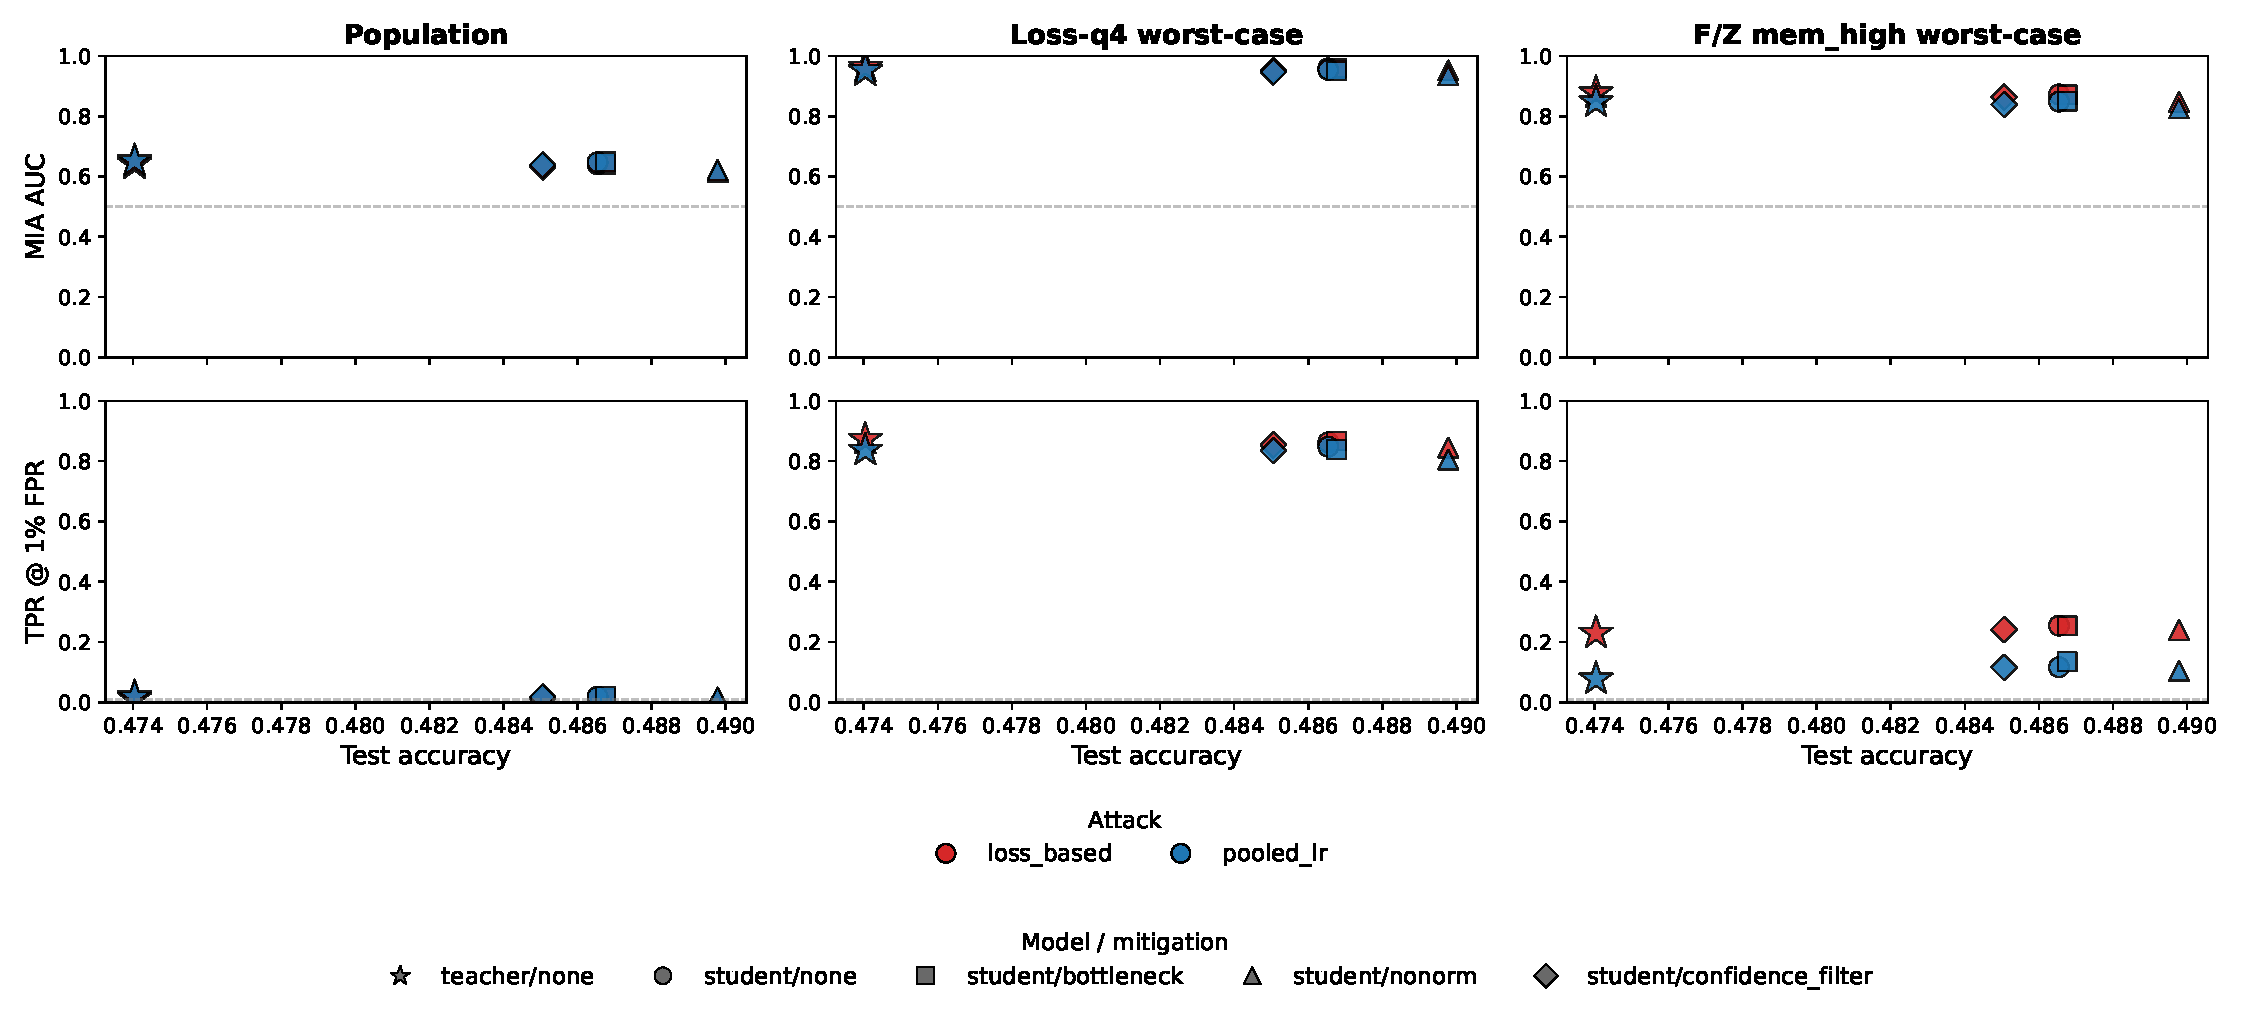
\includegraphics[width=0.95\textwidth]{privacy_utility_comparison.pdf}
\caption{Privacy and utility comparison. The top row reports membership inference AUC and the bottom row reports true-positive rate at $1\%$ false-positive rate. The leftmost column shows the population result, the middle column shows the worst quartile by per-sample teacher loss, and the rightmost column shows the worst bin by Feldman and Zhang memorization. Marker shape encodes the model variant and color encodes the attack. The headline observation is that the mitigation variants are visually indistinguishable in the population view (bottom-left) but separate by an order of magnitude on the memorized long tail (bottom-right), and this separation is the substantive privacy comparison that the population view obscures.}
\label{fig:comparison}
\end{figure*}

\section*{Limitations and Concessions}

The findings above are constrained by the scope of the evaluation in several ways, which the rest of this section enumerates.

The results come from a single dataset, Texas-100X, and a single architecture family of tabular multi-layer perceptrons. A reproduction on Purchase-$100$ would test the dataset assumption. A ResNet teacher distilled into a smaller convolutional student on CIFAR-$100$ would test the architecture assumption. Without one of those, the claim is a property of this particular configuration rather than a general property of knowledge distillation.

The distilled student is undertuned relative to the teacher. The progress report set a target test accuracy of $40\%$ to $45\%$. The alpha sweep, the larger backbone, and the new learning-rate schedule together landed the student at $37.8\%$, against the teacher at $47.4\%$. A reviewer can reasonably argue that the disparate-impact gap is partly confounded with student incapacity, and that a more competent student would leak more. That is the strongest criticism the current evaluation cannot fully rebut. It is worth noting, however, that the direction of the confound favors the thesis rather than undermining it. A more competent student would by construction learn more of the long-tail samples it currently fails to fit, which would in turn raise its long-tail membership inference vulnerability rather than lower it. The population gap between teacher and student would shrink, the long-tail leakage would grow, and the disparate-impact gap reported here is therefore most plausibly a lower bound rather than an artifact.

The high-memorization Feldman and Zhang bin contains $196$ samples for the student variants and $49$ for the teacher. At a $1\%$ false-positive rate on $49$ samples the attack is allowed roughly zero false positives, so the teacher's $0\%$ true-positive rate is sample-size noise rather than a meaningful zero. Bootstrap confidence intervals on the worst-case metrics should accompany any external submission of this work, in line with the more rigorous low-FPR evaluation methodology that Carlini et al.~\cite{carlini2022} advocate for membership inference more generally.

The full Likelihood Ratio Attack was implemented and run with $K = 64$ reference models, each trained on a random $50\%$ subsample for $5$ epochs. Its AUC of $0.503$ on the teacher is below that of the approximate LiRA at $0.652$. This is not a contradiction of the attack literature. It is a known sample-complexity effect. The full attack fits a per-sample Gaussian from the in-set and out-of-set reference confidences, and at $K = 64$ each fit is estimated from roughly $32$ observations per side. The variance of that fit is large enough that the resulting likelihood ratio is no more discriminative on average than the coarser approximate fit, which pools across samples. Carlini et al.~\cite{carlini2022} run their main experiments at $K = 256$ shadow models, and per-sample fits become substantially noisier at smaller $K$. Reproducing the full attack at $K \geq 256$ would require about $4\times$ the reference-model compute already spent here, and is the most obvious extension. The Feldman and Zhang memorization scores use the same reference cache, so the same sample-complexity caveat applies to the absolute $\widehat{\mathrm{mem}}(x)$ values. The sample-level ranking, which is what the stratification depends on, is more robust to the cache size than the absolute values are.

The framing in this paper is borrowed from the disparate-impact critique of differential privacy. The evaluation does not, however, include a comparison against differentially private training. The cleanest extension is to run DP-SGD at moderate $\varepsilon$ on the same dataset and ask whether its subgroup profile is more favorable than knowledge distillation's. That is the obvious next experiment.

\section*{Broader Implications and Ethical Considerations}

The empirical scope of this work is one tabular healthcare dataset and one architecture family. The structural argument is not specific to either. Knowledge distillation is increasingly used in production deployments as a compression technique, and the privacy auditing literature that informs procurement decisions reports population-level attack metrics. An operator deploying a distilled model on the basis of a published average AUC reduction may be making a privacy claim that does not hold for the subgroup of users whose membership is most worth protecting.

The pattern observed here depends on the presence of a long tail in the training distribution, which is a description that fits many domains beyond clinical procedure prediction. Genomics datasets are full of rare variants that a model can only learn by memorization. Financial fraud detection takes individual unusual transactions to be the entire signal of interest. The same structural problem shows up in criminal-justice risk assessment whenever a defendant presents with an atypical case profile. In any setting like these, the population-level privacy metric in an audit report is going to be dominated by the well-classified majority, and the residual identifiability of the long-tail records will not show up in the metric.

One framing caveat worth surfacing is that statistical rarity is not the same property as real-world sensitivity. A rare procedure code may correspond to a vulnerable patient, but it may also correspond to a noisy or mislabeled record whose disclosure carries no particular harm. The argument made here is the narrower one that the subgroup the standard evaluation declares safe is in fact the subgroup the standard evaluation has the least information about. Where the rare subgroup also happens to be the population most in need of protection, as is often the case in healthcare and genomics, the gap between the population metric and the per-record threat becomes a policy concern as well as a methodological one.

Distillation is often pitched as a tradeoff-free defense, since the same operation that compresses the model also reduces the population attack metric. The findings here suggest a sharper framing. Distillation buys an aggregate privacy number. The cost of that purchase is borne disproportionately by the records the aggregate cannot see. A practitioner who selects distillation under the assumption that it provides uniform protection is making a tradeoff that the standard evaluation conceals from them. Technical reports and deployment-side documentation should publish subgroup metrics directly, so that the privacy claim being made on behalf of an operator matches the privacy claim the evaluation actually supports.

There is also a tradeoff between informal defenses like distillation and formal mechanisms like differential privacy. Distillation is cheap to deploy, requires no explicit $\varepsilon$ to negotiate with regulators, and produces a smaller model as a side benefit. Differential privacy goes the other way, offering a per-sample worst-case guarantee at a utility cost that scales sharply as $\varepsilon$ shrinks. The results in this paper say the two are not interchangeable. Distillation does not substitute for the per-sample guarantee that DP provides, even when the two population metrics look comparable. Treating them as substitutes in a procurement context misrepresents the actual privacy posture of the deployed system.

The Bagdasaryan critique of differential privacy raised the concern that the cost of formal guarantees fell disproportionately on underrepresented subgroups. The pattern here is the contrapositive. The benefit of an informal defense accrues disproportionately to the records that were already safe. Averaged across the training set, AUC reduction may look like a privacy improvement. For a single patient with a rare condition that average is largely irrelevant. The model still discloses their membership at a rate one to two orders of magnitude above the published number. Any meaningful evaluation of a privacy defense in a long-tailed setting must therefore report subgroup metrics, not treat the population mean as a sufficient statistic for the privacy claim. The case is sharpest in healthcare, since the long-tail population there is also the population whose data is most sensitive and whose ability to opt out of secondary use is most constrained.

\section*{Conclusion}

The population-level finding that knowledge distillation reduces membership inference vulnerability reproduces faithfully on Texas-100X. The subgroup finding does as well. The largest gains accrue to samples that were never very vulnerable in the first place, and the high-risk subgroups retain nearly all of their leakage. The result holds under three different stratifying signals (per-sample teacher loss, class frequency, and an independently estimated Feldman and Zhang memorization score), so it is not an artifact of any single binning criterion. The three mitigation variants tested look essentially identical at the population level but diverge by an order of magnitude on the memorized long tail. Confidence-filtered distillation appears to actually reduce long-tail leakage. Removing batch normalization appears to make it worse.

The knowledge distillation literature, as currently evaluated, does not deliver uniformly private models. It delivers more-private \emph{averages}. Those averages obscure the patients whose privacy actually depends on a defense. Patients with rare conditions or unusual feature combinations, who are the ones the teacher memorized in the first place, remain nearly as identifiable in the student as in the teacher.

The student fit needs additional tuning, ideally landing in the $40\%$ to $45\%$ accuracy window the progress report set out as a credibility threshold. Bootstrap confidence intervals on the worst-case true-positive rates should be added, since the high-memorization bin is small enough that point estimates are noisy. The full Likelihood Ratio Attack should be re-run with at least $256$ reference models if compute permits. A second dataset and a second architecture pair, plus a DP-SGD baseline, would be needed to push this past the course-project scope into something that stands as a research contribution rather than an empirical case study.

\section*{Reproducibility}

All source code, configuration files, and the canonical artifact directory are available at \url{https://github.com/tgulur/EEP509-Project}. The numerical results and figures in this paper were produced from a single end-to-end pipeline run.

\section*{Acknowledgment and AI Note}

Claude Code was used throughout the project to assist with debugging and clarifying technical concepts. Cursor AI was used to scaffold the initial file structure of the codebase at the outset of the course. Claude Code was additionally employed to write test cases and establish a set of project constraints to ensure robustness of the pipeline against unintended modifications.

\begin{thebibliography}{00}

\bibitem{shokri2017} R. Shokri, M. Stronati, C. Song, and V. Shmatikov, ``Membership inference attacks against machine learning models,'' in \emph{Proc. IEEE Symp. Security and Privacy (S\&P)}, 2017, pp. 3--18. \url{https://arxiv.org/abs/1610.05820}

\bibitem{yeom2018} S. Yeom, I. Giacomelli, M. Fredrikson, and S. Jha, ``Privacy risk in machine learning: Analyzing the connection to overfitting,'' in \emph{Proc. IEEE Computer Security Foundations Symp. (CSF)}, 2018, pp. 268--282. \url{https://arxiv.org/abs/1709.01604}

\bibitem{bagdasaryan2019} E. Bagdasaryan, O. Poursaeed, and V. Shmatikov, ``Differential privacy has disparate impact on model accuracy,'' in \emph{Advances in Neural Information Processing Systems (NeurIPS)}, 2019. \url{https://arxiv.org/abs/1905.12101}

\bibitem{feldman2020} V. Feldman and C. Zhang, ``What neural networks memorize and why: Discovering the long tail via influence estimation,'' in \emph{Advances in Neural Information Processing Systems (NeurIPS)}, 2020. \url{https://arxiv.org/abs/2008.03703}

\bibitem{carlini2022} N. Carlini, S. Chien, M. Nasr, S. Song, A. Terzis, and F. Tram\`er, ``Membership inference attacks from first principles,'' in \emph{Proc. IEEE Symp. Security and Privacy (S\&P)}, 2022. \url{https://arxiv.org/abs/2112.03570}

\bibitem{shejwalkar2021} V. Shejwalkar and A. Houmansadr, ``Membership privacy for machine learning models through knowledge transfer,'' in \emph{Proc. AAAI Conf. Artificial Intelligence}, 2021. \url{https://arxiv.org/abs/1906.06589}

\bibitem{tang2022} X. Tang, S. Mahloujifar, L. Song, V. Shejwalkar, M. Nasr, A. Houmansadr, and P. Mittal, ``Mitigating membership inference attacks by self-distillation through a novel ensemble architecture,'' in \emph{Proc. USENIX Security Symposium}, 2022. \url{https://arxiv.org/abs/2110.08324}

\bibitem{texas100x} B. Jayaraman, ``Texas-100X dataset.'' \url{https://github.com/bargavj/Texas-100X}

\end{thebibliography}

\end{document}
